% This file was created with tikzplotlib v0.10.1.
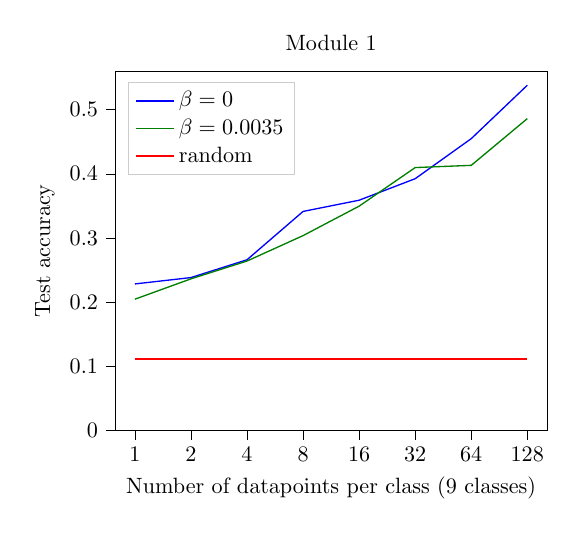
\begin{tikzpicture}[scale=0.8]

\definecolor{darkgray176}{RGB}{176,176,176}
\definecolor{green01270}{RGB}{0,127,0}
\definecolor{lightgray204}{RGB}{204,204,204}

\begin{axis}[
	legend cell align={left},
	legend style={
		fill opacity=0.8,
		draw opacity=1,
		text opacity=1,
		at={(0.03,0.97)},
		anchor=north west,
		draw=lightgray204
	},
	log basis x={2},
	tick align=outside,
	tick pos=left,
	title={Module 1},
	x grid style={darkgray176},
	xlabel={Number of datapoints per class (9 classes)},
	xmin=0.784584097896751, xmax=163.143760296865,
	xmode=log,
	%	%	xtick={0,1,2,3,5,6,7}, % <-- Modify xtick values here
	%		xtick={0,0.30103,0.60206,0.90309,1.50515,1.80618,2.10721}, % <-- Adjusted xtick values
	xticklabels={0, 1,2,4,8,16, 32,64,128}, % <-- Modify xtick labels here
	xtick style={color=black},
	y grid style={darkgray176},
	ylabel={Test accuracy},
	ymin=0.0, ymax=0.559548593309191,
	ytick style={color=black}
	]
\addplot [semithick, blue]
table {%
1 0.228174594470433
2 0.238095226969038
4 0.265873006411961
8 0.341269825526646
16 0.35879628499349
32 0.392361106872559
64 0.454861106872559
128 0.538194427490234
};
\addlegendentry{$\beta = 0$}
\addplot [semithick, green01270]
table {%
1 0.20436507156917
2 0.236111101422991
4 0.263888878141131
8 0.303571417672294
16 0.349537022908529
32 0.409722213745117
64 0.413194427490234
128 0.486111106872559
};
\addlegendentry{$\beta = 0.0035$}
\addplot [semithick, red]
table {%
1 0.111111111111111
2 0.111111111111111
4 0.111111111111111
8 0.111111111111111
16 0.111111111111111
32 0.111111111111111
64 0.111111111111111
128 0.111111111111111
};
\addlegendentry{random}
\end{axis}

\end{tikzpicture}
